%%%%%%%%%%%%%%%%%%%%%%%%%%%%%%%%%%%%%%%%%%%%%%%%%%%%%%%%%%%%%%%%%%%%
% Trello API wrapper
%%%%%%%%%%%%%%%%%%%%%%%%%%%%%%%%%%%%%%%%%%%%%%%%%%%%%%%%%%%%%%%%%%%%
\onehalfspacing
\chapter{Trello API wrapper}\index{Trello}\index{API}

These scripts fulfill very different tasks, but they have also much in common. For example almost every script potentially loads single cards. This API wrapper represent Trello in Ruby. This is a kind of translation from Trello to Ruby and vice versa. Additionally, now the scripts can use the functions and in consequence they can stay very lightweight and clean. Almost everything that's possible with the Trello API is also possible with this API wrapper. But it doesn't cover all features, because the API is still in beta phase, so it changes quite quickly.

\begin{figure}
\centering
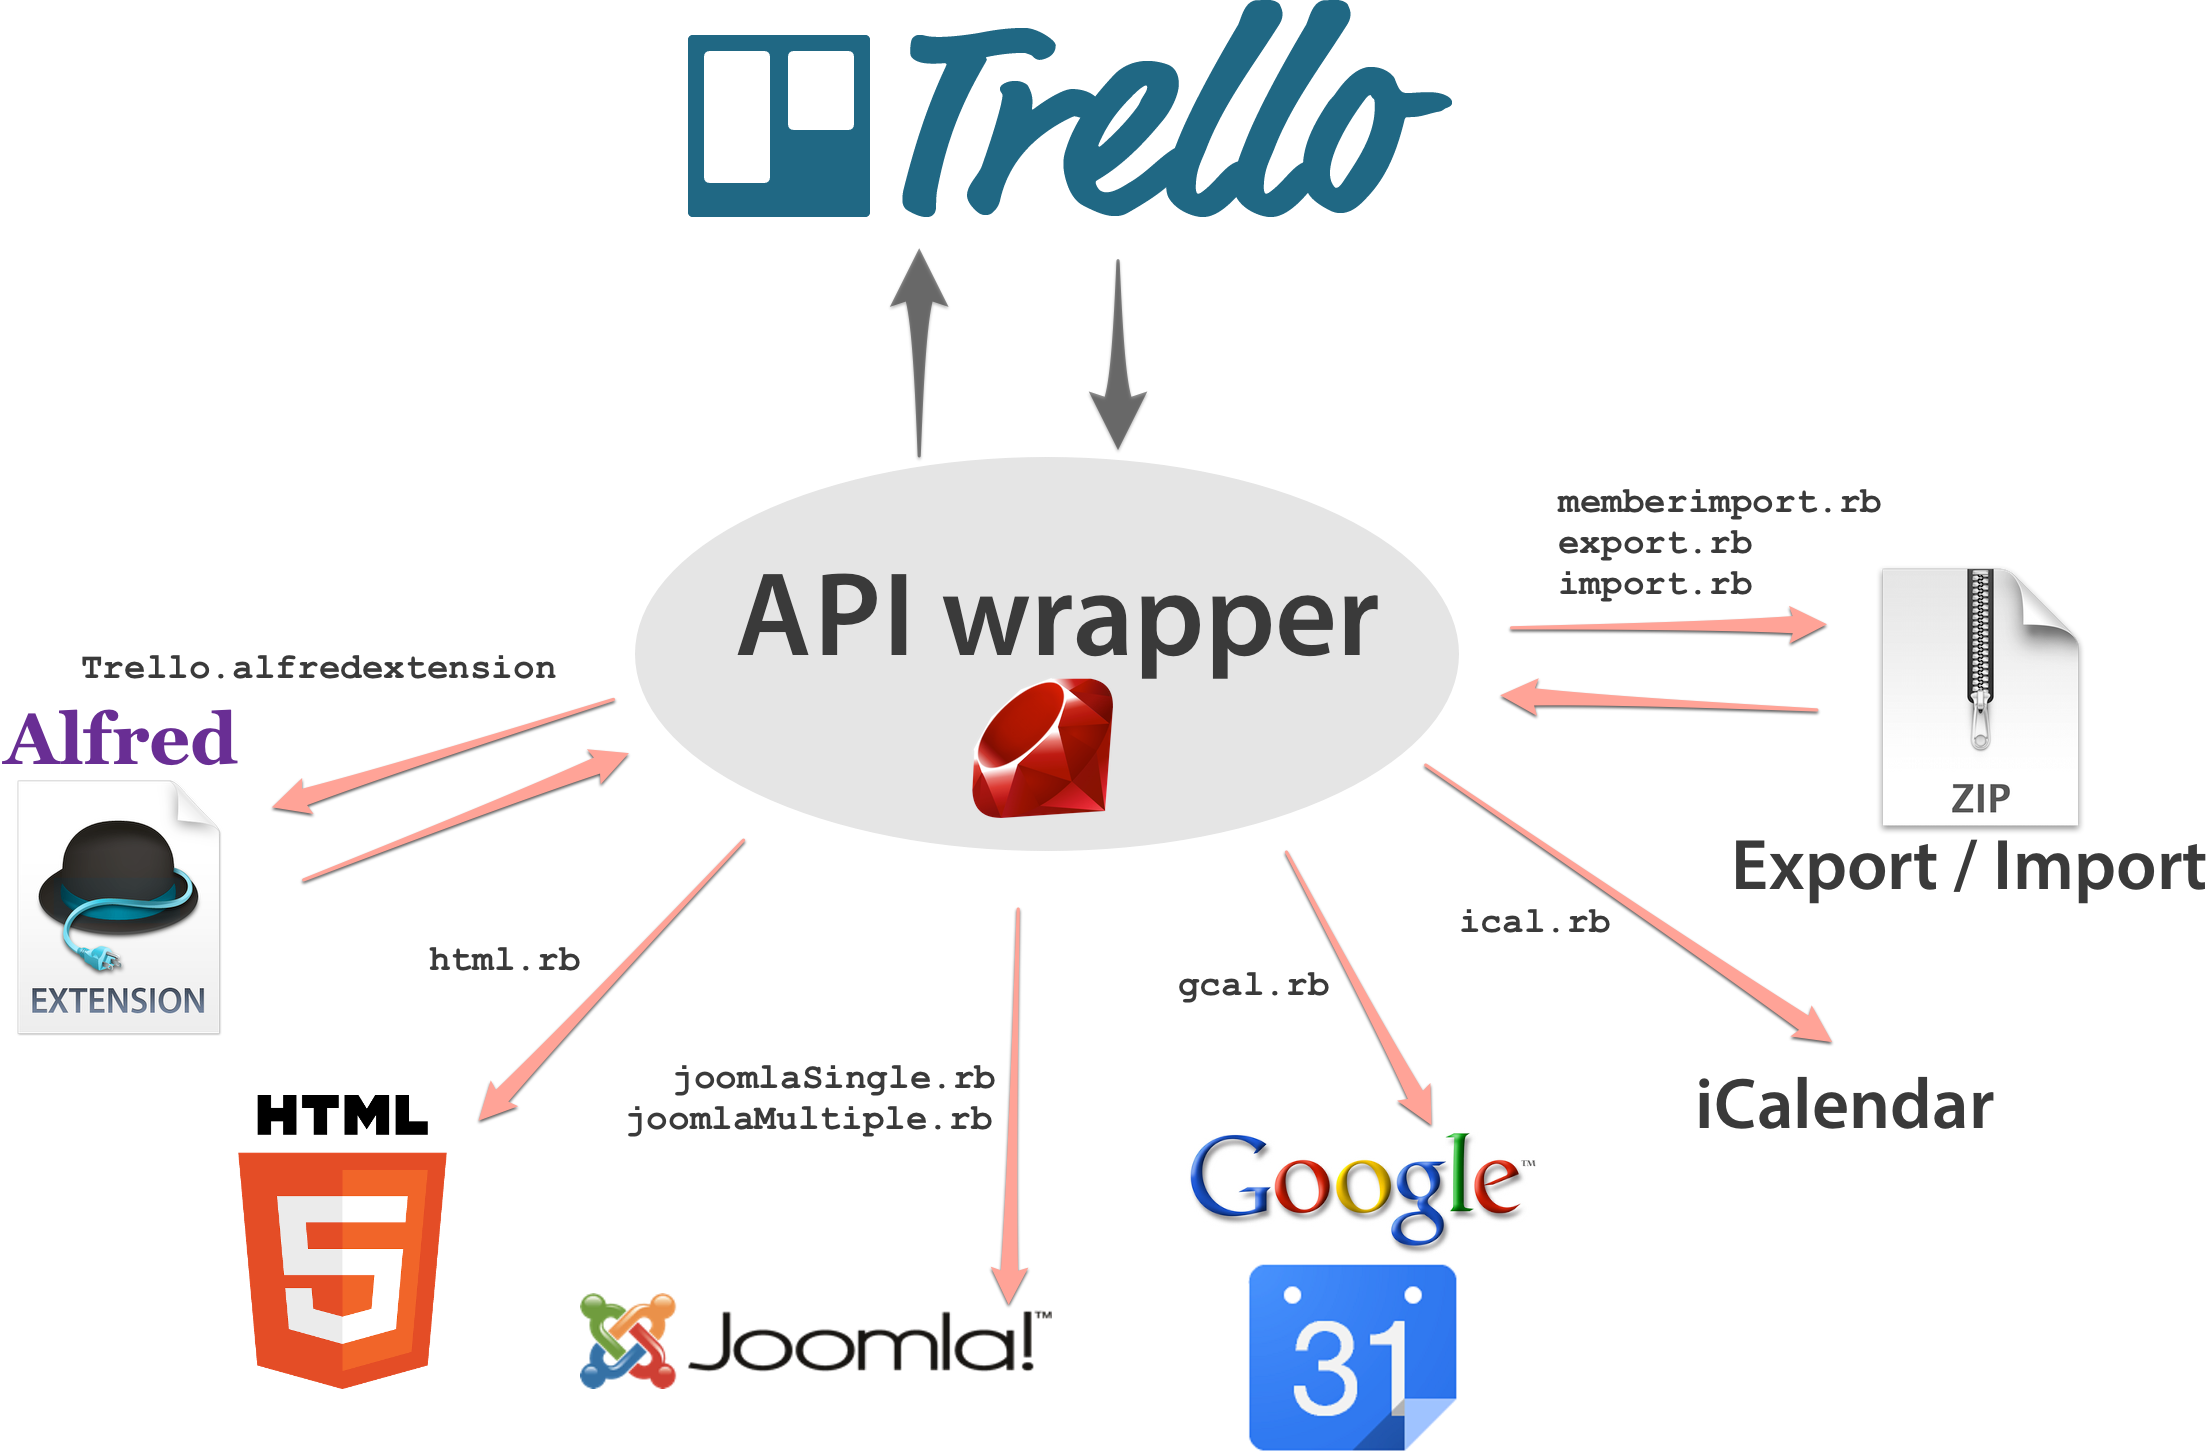
\includegraphics[width=\textwidth]{figures/api-wrapper}
\caption{Connections between Trello, the API wrapper and the actual features. \cite{ruby:icon}\cite{html:logo}\cite{joomla}\cite{google} }
\label{fig: api-wrapper}
\end{figure}

The API wrapper also has functions to pre-process data for Ruby. From a developer's point of view, Trello is all about cards. Cards are the only things in Trello with real data, not just meta data. So if the task is to get a board from the API\index{API} it means to get the cards of the board. There is an API call to get all cards which are in a specific board. But with this call the developer doesn't get all the information about the cards. So the API wrapper has to execute the API call for a single card to cumulate all the information about all the cards of the board. This is the function of the API wrapper to keep the actual script clean. So the developer can work with the data and doesn't have to worry about determining it.

\todo{So stehen lassen?} The API wrapper is meant to perform all API calls which are required by the scripts. None of the API calls should be performed by the scripts that use the bucket.

\section{Error handling}
\todo{Error Handling}

Error handling in Ruby is realised with \lstinline{begin} blocks. A \lstinline{begin} block is like an \lstinline{if} expression but for \lstinline{exceptions}. 

\begin{lstlisting}[aboveskip=1\baselineskip, caption=Error handling with \lstinline{begin} blocks., label=listing042]
begin
	my = Mysql.init
	my.real_connect(dbhost, dbuser, dbpassword, db)
rescue => e
	puts e.message
else  (*@ \label{line036} @*)
	puts "It works!"
ensure
	mysql.close if mysql
end
\end{lstlisting}

A \lstinline{begin} block has several section. The first section is the \lstinline{begin} section. Here the code to check is executed. The example in listing \ref{listing042} shows a simple database connection. With the \lstinline{begin} block araound it Ruby checks if there occur any exceptions while executing this code. If there are exception indeed, the \lstinline{rescue} sections comes to help out. The error is stored in the variable \lstinline{e}. At least the message can be printed here, to inform the user. A \lstinline{begin} block may contain multiple \lstinline{rescue} sections. It's possible to specify special types of exceptions so corresponding actions can be performed. 

\begin{lstlisting}[aboveskip=1\baselineskip, caption=\texttt{joomlaMultiple.rb} usage., label=listing043]
rescue Mysql::Error => e
\end{lstlisting}

In listing \ref{listing043} the \lstinline{Mysql::Error} class is specified. In this \lstinline{rescue} section only exception of this class will be handled.

An \lstinline{else} section in a \lstinline{begin} block like in \ref{line036} of listing \ref{listing042} is allowed only if there is one or more \lstinline{rescue} blocks. It is executed if there are no exceptions. The last section is the \lstinline{ensure} block. It is executed no matter whether there is an exception or not. In the example the initialiser database connection is closed. This section is supposed to finish the execution of the whole block.


\section{Command Line Interface}\nomenclature{CLI}{Command Line Interface}\index{CLI}\index{Command-Line Interface}\label{cli}
Almost every script needs some information. The information which every scripts needs is the key and token of the user whose account should be used to access Trello. The scripts have to know which cards, lists and boards they have to look at. So this information has to be passed on to the scripts, too. At first we set this information at the top of the script. But it emerged that it's very unpractical to hard code this in each script. So it would be impossible to use the same Ruby file with several Trello accounts. For every Trello account the user has to generate a dedicated file. The solution for this problem is a command-line interface (CLI). With a CLI the user can pass on information to the script in a predefined format, so the script knows exactly what to do. For every other call the user can specify different information for the same script.

The Ruby class OptionParser\cite{ruby:optionparser} provides easy customisable command-line option analysis. The developer is able to specify its own options for each script. For this purpose a dedicated class is used. 
In order to let the actual script \emph{know} about the CLI arguments the developer has to require the respective CLI class with the command-line option definitions.

\begin{lstlisting}[aboveskip=1\baselineskip, style=bash, caption=Example usage of a script with CLI., label=listing004]
ruby html.rb -c 4ffd78a2c063afeb066408b8
\end{lstlisting}

An example usage of a script with CLI would look like Listing \ref{listing004}. The \texttt{-c} is a command-line option. If there is a string behind the option, like in this case, the string is a so called \emph{argument}. But there are command-line options which stand by themselves. These are called \emph{flags}. Flags are only for polar decisions.

\begin{lstlisting}[aboveskip=1\baselineskip, caption=Definition of a command-line option, label=listing002]
# Trello list(s)
opts.on("-l", "--lists x,y,z", Array, "Ids of one or more Trello lists.") do |lists| (*@\label{line001}@*)
	options.lists = lists
end
\end{lstlisting}

Listing \ref{listing002} shows the definition of the option \texttt{-l} for passing one or more IDs of lists to a script. In Line \ref{line001} the word \lstinline{Array} casts the list argument to an Array object.

OptionParse provides an automated help option. If the user types 
\begin{center}
\texttt{ruby script.rb -h} 
\end{center}
he gets the explanation the developer wrote in the CLI class for this script with all possible options. This list is automatically generated by the definitions of the command-line options like in Listing \ref{listing002}. It works with \texttt{-help} and \texttt{--help} instead of \texttt{-h}, too.

\begin{lstlisting}[aboveskip=1\baselineskip, style=bash, caption=Output of the \texttt{-h} option., label=listing003]
Usage: ical.rb [options]
Select the input cards with -c, -l, -b or -a

Specific options:
 -a, --[no-]all         Set this if all due dates of all cards of all boards this user can see shall be used.
 -l, --lists x,y,z      Ids of one or more Trello lists.
 -b, --boards x,y,z     Ids of one or more Trello boards.
 -c, --cards x,y,z      Ids of one or more Trello cards.
 -k MANDATORY, --key    Your Trello key.
 -t MANDATORY, --token  The Trello token.
\end{lstlisting}

Listing \ref{listing003} shows the Output of \texttt{ruby ical.rb -h}. 
These are the basic CLI commands used by every script. For some scripts there are additional commands. They are explained in their respective sections.

\section{Actual methods} \todo{Working title!!!}
The API calls which are wrapped by the following methods need a private key and a token to access content in private boards. Thus, private key and token need not be sent to each method, it will be initialized in each script as global variables. The variable for the private key is alled \lstinline{$key} and the one for the token is called \lstinline{$token}.

\subsection{Handling of date and time}
Content in Trello may have set dates. These dates are represented by the Trello API as an ISO\nomenclature{ISO}{International Organization for Standardization} 8601\index{ISO!8601}\footnote{More information about ISO 8601 on the website of the International Organization for Standardization: \url{http://www.iso.org/iso/home/store/catalogue_tc/catalogue_detail.htm?csnumber=40874}. The RFC 3339 is a profile of ISO 8601: \url{http://www.ietf.org/rfc/rfc3339.txt}} formatted string. The timezone\index{timezone} of the date is UTC\nomenclature{UTC}{Universal Time Coordinated}. To ensure that the correct time is always displayed the date has to be adapted to the local time. 

\subsubsection{getDate(date, format='de')}
\begin{lstlisting}[aboveskip=1\baselineskip, caption=\lstinline{getDate()}, label=listing044]
def getDate(date, format='de')
	fdate = Time.iso8601(date).getlocal (*@ \label{line045} @*)
	
	if format=='de'
		return fdate.strftime('%d.%m.%Y %H:%M:%S')
	elsif format=='us'
		return fdate.strftime('%m/%d/%Y %I.%M.%S %P')
	elsif format=='joomla'
		return fdate.strftime('%Y-%m-%d %H:%M:%S')
	elsif format=='ical'
		return fdate.strftime('%Y%m%dT%H%M%S')
	elsif format=='year'
		return fdate.strftime('%Y')
	elsif format=='iso8601'
		return fdate.iso8601
	end
end
\end{lstlisting}

In line \ref{line045} of listing \ref{listing044} the given date string in ISO 8601 format is parsed to a Ruby Time object. The \lstinline{getlocal} is the important part here. This function of the Time class determines the server's time zone and readjusts the time accordingly. The method respects the daylight saving time in several time zones, too. For this function working as intended it's important that the correct time zone is set on the used server. 

The \lstinline{getDate()} method additionaly converts the date to othe formats. 

\subsection{Collect data from Trello}
The several objects in Trello such as cards, lists and boards are accessed by these scripts regularly. To keep the actual scripts clean the API wrapper includes methods to determine and process the information of these onjects.

\subsubsection{getBoardsByMember(memberId)}
\begin{lstlisting}[aboveskip=1\baselineskip, caption=\lstinline{getBoardsByMember()}, label=listing045]
def getBoardsByMember(memberId)
	boards = RestClient.get("https://api.trello.com/1/members/"+memberId+"/boards?key="+$key+"&token="+$token+"&filter=open")
	boards = JSON.parse(boards)
end
\end{lstlisting}
The method \lstinline{getBoardsByMember()} receives a member id and determines all boards accessible by this Trello account.

\subsubsection{getListsByBoard(boardId)}
\begin{lstlisting}[aboveskip=1\baselineskip, caption= getListsByBoard(), label=listing046]
def getListsByBoard(boardId)
	list = RestClient.get("https://api.trello.com/1/boards/"+boardId+"/lists?key="+$key+"&token="+$token)
	list = JSON.parse(list)	
end
\end{lstlisting}

\subsubsection{getList(listId)}
\begin{lstlisting}[aboveskip=1\baselineskip, caption= getList(), label=listing047]
def getList(listId)
	list = RestClient.get("https://api.trello.com/1/lists/"+listId+"?key="+$key+"&token="+$token)
	list = JSON.parse(list)	
end
\end{lstlisting}

\subsubsection{getSingleCard(cardId)}
\begin{lstlisting}[aboveskip=1\baselineskip, caption=getSingleCard(), label=listing048]
def getSingleCard(cardId)
	card = RestClient.get("https://api.trello.com/1/cards/"+cardId+"?key="+$key+"&token="+$token)
	card = JSON.parse(card)
end
\end{lstlisting}

\subsubsection{getCardsByBoard(boardId)}\begin{lstlisting}[aboveskip=1\baselineskip, caption=getCardsByBoard() label=listing049]
def getCardsByBoard(boardId)
	board = RestClient.get("https://api.trello.com/1/boards/"+boardId+"/cards?key="+$key+"&token="+$token+"&filter=open")
	board = JSON.parse(board)
end
\end{lstlisting}

\subsubsection{getCardsByList(listId)}
\begin{lstlisting}[aboveskip=1\baselineskip, caption=getCardsByList(), label=listing050]
def getCardsByList(listId)
	list = RestClient.get("https://api.trello.com/1/lists/"+listId+"/cards?key="+$key+"&token="+$token+"&filter=open")
	list = JSON.parse(list)
end
\end{lstlisting}

\subsubsection{getCardsAsArray(arrayCardsStd, downloads = true)}
\begin{lstlisting}[aboveskip=1\baselineskip, caption= getCardsAsArray(), label=listing063]
def getCardsAsArray(arrayCardsStd, downloads = true)
	arrayCardsFull = Array.new
	directoryNameAttachments = File.join(Dir.tmpdir, "attachments")
	
	arrayCardsStd.each do |card|
		# export members
		memberArray = Array.new
		card['idMembers'].each do |memberId|
			member = getMember(memberId)
			memberArray << member			
		end
		membersForCard = Hash.new
		membersForCard['members'] = memberArray
		card = card.merge(membersForCard)
		# end export members		
		
		# export checklists
		hasChecklist = getChecklist(card['id']) 
		
		if hasChecklist[0] != nil
			arrayChecklists = Array.new
			hasChecklist.each do |checklist|  
				hashChecklist = Hash.new  
				hashChecklist['id'] = checklist['id']
				hashChecklist['name'] = checklist['name']
				arrayItems = Array.new
				checklist['checkItems'].each do |item|
					hashItem = Hash.new
					hashItem['name'] = item['name']
					if isCompleted(card['id'], item['id'])
						hashItem['completed'] = true
					else
						hashItem['completed'] = false
					end
					hashItem['pos'] = item['pos']
					arrayItems.push(hashItem)
				end
				hashChecklist['items'] = arrayItems
				arrayItems = nil
				arrayChecklists.push(hashChecklist)
				hashChecklist = nil
			end
			
			hashCheckListsForCard = Hash.new
			hashCheckListsForCard['checklists'] = arrayChecklists
			
			card = card.merge(hashCheckListsForCard)
		end
		# end export checklists
		
		# export comments
		if card['badges']['comments'] != 0
			comments = getCardComments(card['id'])
			hashCommentsForCard = Hash.new			
			hashCommentsForCard['commentsContent'] = comments			
			card = card.merge(hashCommentsForCard)
		end
		# end export comments
		
		# export attachments
		if card['badges']['attachments'] != 0
			attachments = getAttachment(card['id'])			
			hashAttachmentsForCard = Hash.new			
			hashAttachmentsForCard['attachments'] = attachments			
			card = card.merge(hashAttachmentsForCard)			
			
			if downloads
				# url runterladen
				attachments.each do |attachment|
					fileDomain = URI.parse(attachment['url']).host
					filePath = attachment['url'].gsub(URI.parse(attachment['url']).scheme+"://"+URI.parse(attachment['url']).host, '')
					fileExtension = File.extname(attachment['url'])
					
					fileName = attachment['id']+File.basename(attachment['url'])
					puts "Downloading \'"+fileName+"\'"
								
					if !Dir.exists?(directoryNameAttachments)
						Dir::mkdir(directoryNameAttachments)
					end
					
					Net::HTTP.start(fileDomain) do |http|
							resp = http.get(filePath)
							open(directoryNameAttachments+"/"+fileName, "wb") do |file|
									file.write(resp.body)
							end
					end      
				end
				# url runterladen
			end       
		end	
		# end export attachments
		
		# export votes
		if card['badges']['votes'] > 0
			reply = RestClient.get(
					'https://api.trello.com/1/cards/'+card['id']+'/membersVoted?key='+$key+'&token='+$token
			)
			members = JSON.parse(reply)
			membersVotedArray = Array.new
			members.each do |member|
				 membersVotedArray.push(member['id'])
			end
			hashMembersVotedForCard = Hash.new			
			hashMembersVotedForCard['membersVoted'] = membersVotedArray
			card = card.merge(hashMembersVotedForCard)	
		end
		# end export votes
		
		arrayCardsFull.push(card)
	end
	
	return arrayCardsFull
end
\end{lstlisting}

\todo{Describe all the methods. Consider renaming for constancy?}

\subsection{Further information on a card}

\subsubsection{getCardActions(cardId)}
\begin{lstlisting}[aboveskip=1\baselineskip, caption=getCardActions(), label=listing051]
def getCardActions(cardId)
	actions = RestClient.get("https://api.trello.com/1/cards/"+cardId+"/actions?key="+$key+"&token="+$token)
	actions = JSON.parse(actions)
end
\end{lstlisting}

\subsubsection{getCardComments(cardId)}
\begin{lstlisting}[aboveskip=1\baselineskip, caption= getCardComments(), label=listing052]
def getCardComments(cardId)
	actions = RestClient.get("https://api.trello.com/1/cards/"+cardId+"/actions?filter=commentCard&key="+$key+"&token="+$token)
	actions = JSON.parse(actions)
end
\end{lstlisting}

\subsubsection{cardUpdated(cardId)}
\begin{lstlisting}[aboveskip=1\baselineskip, caption= cardUpdated(), label=listing053]
def cardUpdated(cardId)
	reply = RestClient.get('https://api.trello.com/1/cards/'+cardId+'/actions?filter=updateCard&key='+$key+'&token='+$token)

	updates = JSON.parse(reply.body)
end
\end{lstlisting}

\subsubsection{cardCreated(cardId)}
\begin{lstlisting}[aboveskip=1\baselineskip, caption= cardCreated(), label=listing054]
def cardCreated(cardId)
	reply = RestClient.get('https://api.trello.com/1/cards/'+cardId+'/actions?filter=createCard&key='+$key+'&token='+$token)

	updates = JSON.parse(reply.body)
end
\end{lstlisting}

\subsubsection{isCompleted(cardId, itemId)}
\begin{lstlisting}[aboveskip=1\baselineskip, caption= isCompleted(), label=listing055]
def isCompleted(cardId, itemId)
	completedItems = RestClient.get("https://api.trello.com/1/cards/"+cardId+"/checkitemstates?key="+$key+"&token="+$token)
	completedItems = JSON.parse(completedItems)

	completedItems.each do |item|
		if item['idCheckItem'] == itemId
			return true
		end
	end

	return false
end
\end{lstlisting}

\subsubsection{getChecklist(cardId)}
\begin{lstlisting}[aboveskip=1\baselineskip, caption= getChecklist(), label=listing056]
def getChecklist(cardId)
	checklists = RestClient.get("https://api.trello.com/1/cards/"+cardId+"/checklists?key="+$key+"&token="+$token)
	data = JSON.parse(checklists)

	return data  
end
\end{lstlisting}

\subsubsection{getAttachment(cardId)}
\begin{lstlisting}[aboveskip=1\baselineskip, caption= getAttachment(), label=listing057]
def getAttachment(cardId)
	attachments = RestClient.get("https://api.trello.com/1/cards/"+cardId+"/attachments?key="+$key+"&token="+$token)
	data = JSON.parse(attachments)

	return data
end
\end{lstlisting}

\todo{Describe all the methods. Consider renaming for constancy?}

\subsection{Member information}

\subsubsection{getMember(memberId)}
\begin{lstlisting}[aboveskip=1\baselineskip, caption= getMember(), label=listing058]
def getMember(memberId)
	member = RestClient.get("https://api.trello.com/1/members/"+memberId+"?key="+$key+"&token="+$token+"&filter=open")
	member = JSON.parse(member)
end
\end{lstlisting}

\subsubsection{isThisMe(memberId)}
\begin{lstlisting}[aboveskip=1\baselineskip, caption= isThisMe(), label=listing059]
def isThisMe(memberId)
	if getMember('me')['id'] == memberId
		return true
	else
		return false
	end
end
\end{lstlisting}

\subsubsection{getMembersByBoard(boardId)}
\begin{lstlisting}[aboveskip=1\baselineskip, caption= getMembersByBoard(), label=listing060]
def getMembersByBoard(boardId)
	members = RestClient.get("https://api.trello.com/1/boards/"+boardId+"/members?&key="+$key+"&token="+$token)
	members = JSON.parse(members)	
end
\end{lstlisting}

\subsection{Accessing CMS}

\subsubsection{trelloToJoomlaSingle(joomlaArticleId, articles)}
\begin{lstlisting}[aboveskip=1\baselineskip, caption= trelloToJoomlaSingle(), label=listing061]

\end{lstlisting}

\subsubsection{trelloJoomlaSync(cardId, sectionid, catid, joomlaVersion)}
\begin{lstlisting}[aboveskip=1\baselineskip, caption= trelloJoomlaSync(), label=listing062]

\end{lstlisting}




